\documentclass{article}

\usepackage{graphicx}
\usepackage{tikz}
\usepackage{tikzsymbols}
\usetikzlibrary{calc,patterns,shapes.geometric}
\pagestyle{empty}
\usepackage[margin=0pt]{geometry}
\geometry{papersize={14in,12in}}

\def\centerarc[#1](#2)(#3:#4:#5){\draw[#1] ($(#2)+({#5*cos(#3)},{#5*sin(#3)})$) arc (#3:#4:#5);}

\begin{document}
	\begin{figure}
		\centering
		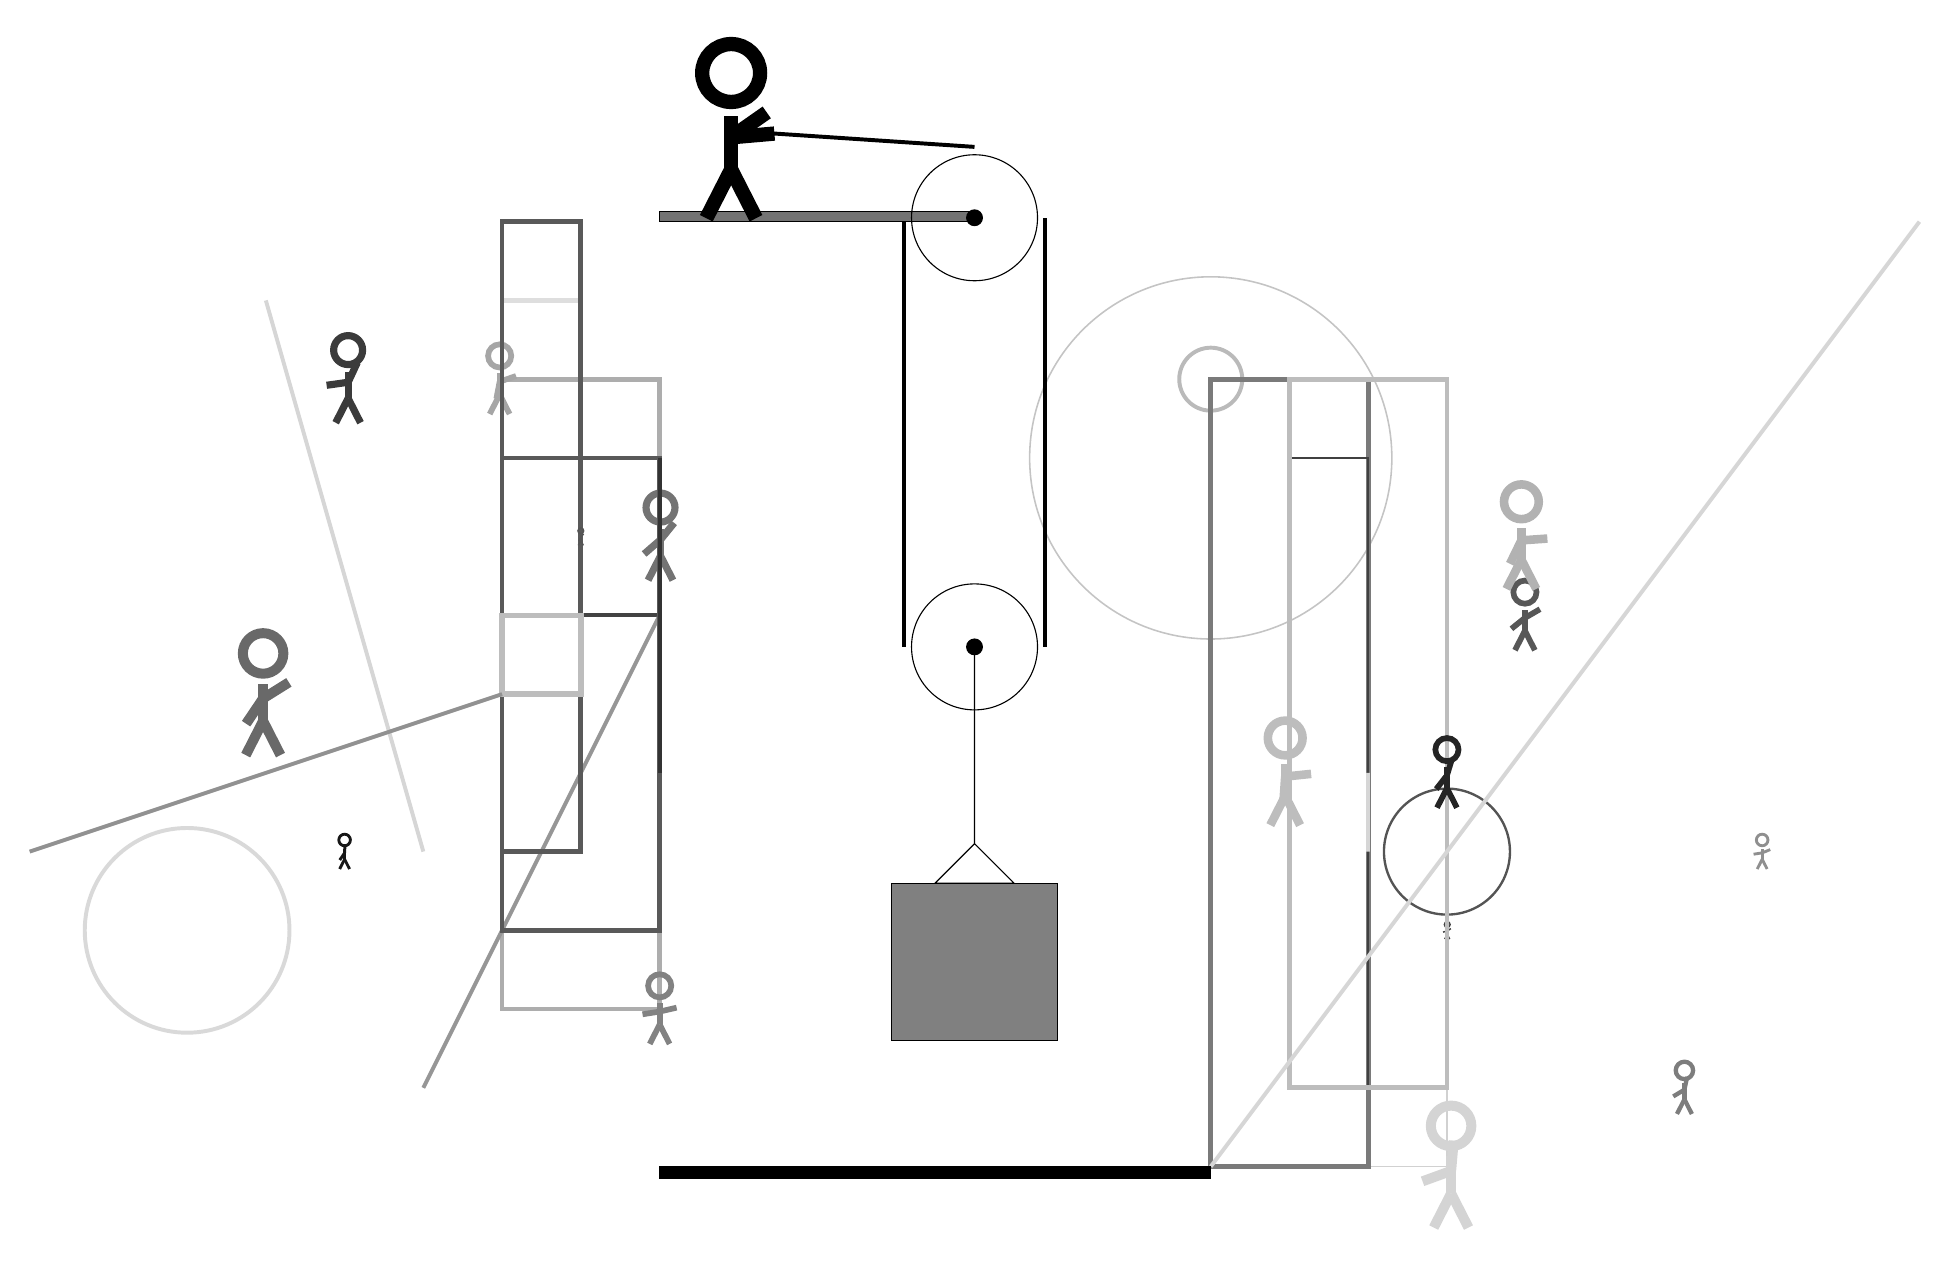
\begin{tikzpicture}
			%%%%% START %%%%%
			
			\draw[fill=black!55] (-2, 9) rectangle (2, 9.125);
			
			\draw (2, 3.6) circle (0.8);
			\draw[fill=black] (2, 3.6) circle (0.1);
			
			\draw (2, 9.05) circle (0.8);
			\draw[fill=black] (2, 9.05) circle (0.1);
			
			\draw (2, 3.6) -- (2, 1.1) -- (1.5, 0.6) -- (2.5, 0.6) -- (2, 1.1);
			\draw[fill=black!50] (0.95, 0.6) rectangle (3.05, -1.4);
			
			\draw[line width=0.5mm, color=black!16](-7, 8) -- (-5, 1);
			
			\draw [line width=0.2mm, color=black!23](5, 6) circle (2.3);
			\node[line width=0.7mm, color=black!59] at (-7, 3) {\Strichmaxerl[7][56][32]};
			\draw[line width=0.5mm, color=black!74] (-3, 4) rectangle (-2, 6);
			\draw[line width=0.2mm, color=black!18] (7, -3) rectangle (8, 7);
			\draw[line width=0.6mm, color=black!32] (-4, -1) rectangle (-2, 7);
			\draw [line width=0.3mm, color=black!67](8, 1) circle (0.8);
			
			\draw[line width=0.6mm, color=black!13] (-3, 6) rectangle (-4, 8);
			\node[line width=0.4mm, color=black!44] at (12, 1) {\Strichmaxerl[2][9][22]};
			\draw[line width=0.6mm, color=black!31] (-4, 7) rectangle (-4, 7);
			
			\node[line width=0.2mm, color=black!55] at (-2, 5) {\Strichmaxerl[5][41][51]};
			\draw[line width=0.5mm, color=black!57](8, 8) -- (8, 8);
			\node[line width=0.2mm, color=black!49] at (-2, -1) {\Strichmaxerl[4][9][13]};
			
			\draw [line width=0.5mm, color=black!27](5, 7) circle (0.4);
			\node[line width=0.6mm, color=black!35] at (-4, 7) {\Strichmaxerl[4][79][19]};
			\draw[line width=0.5mm, color=black!41](-5, -2) -- (-2, 4);
			\draw[line width=0.6mm, color=black!52] (7, 7) rectangle (5, -3);
			\node[line width=0.6mm, color=black!77] at (-6, 7) {\Strichmaxerl[5][8][65]};
			\node[line width=0.6mm, color=black!74] at (8, 0) {\Strichmaxerl[1][15][33]};
			
			\draw[line width=0.6mm, color=black!65] (-4, 6) rectangle (-2, 0);
			\draw[line width=0.2mm, color=black!75] (6, 6) rectangle (7, -2);
			
			\draw[line width=0.5mm, color=black!80] (-2, 2) rectangle (-2, 6);
			
			\node[line width=0.5mm, color=black!91] at (-6, 1) {\Strichmaxerl[2][56][87]};
			\draw[line width=0.6mm, color=black!26] (6, 7) rectangle (8, -2);
			\draw[line width=0.5mm, color=black!16](5, -3) -- (14, 9);
			
			\draw[line width=0.5mm, color=black!16] (7, 2) rectangle (7, 1);
			\node[line width=0.7mm, color=black!66] at (9, 4) {\Strichmaxerl[4][39][30]};
			\node[line width=0.4mm, color=black!30] at (9, 5) {\Strichmaxerl[6][64][4]};
			\node[line width=0.7mm, color=black!26] at (6, 2) {\Strichmaxerl[6][86][6]};
			
			\draw[line width=0.6mm, color=black!65] (-4, 1) rectangle (-3, 9);
			\draw[line width=0.7mm, color=black!26] (-3, 4) rectangle (-4, 3);
			\node[line width=0.5mm, color=black!17] at (8, -3) {\Strichmaxerl[7][20][85]};
			\node[line width=0.3mm, color=black!86] at (8, 2) {\Strichmaxerl[4][52][73]};
			\node[line width=0.7mm, color=black!51] at (11, -2) {\Strichmaxerl[3][31][78]};
			\draw [line width=0.5mm, color=black!15](-8, 0) circle (1.3);
			\node[line width=0.6mm, color=black!67] at (-3, 5) {\Strichmaxerl[1][61][50]};
			\draw[line width=0.5mm, color=black!43](-4, 3) -- (-10, 1);
			
			\draw[line width=0.5mm] (1.1, 9) -- (1.1, 3.6);
			\centerarc[line width=0.5mm](2, 3.6)(180:360:0.9);
			\draw[line width=0.5mm](2.9, 3.6) -- (2.9, 9.05);
			\centerarc[line width=0.5mm](2, 9.05)(0:90:0.9);
			\draw[line width=0.5mm](2, 9.95) -- (-1, 10.15);
			
			\node at (-1, 10.15) {\Strichmaxerl[10][-175][35]};
			
			\draw[fill=black] (-2, -3) rectangle (5, -3.15);
			
			%%%%% END %%%%%
		\end{tikzpicture}
	\end{figure}	
\end{document}